\documentclass[basic, header]{nosvagor-notes}
\usepackage{nosvagor-math}

\colorlet{title-color}{red}
\newcommand{\theTitle}{%
  \href{https://github.com/nosvagor/notes}%
  {Homework 8}%
}

\usepackage{tikz}
\usepackage{qtree}

\newcommand{\userName}{Cullyn Newman}
\newcommand{\class}{CS: 250}
\newcommand{\institution}{Portland State}

\begin{document}
%%%%%%%%%%%%%%%%%%%%%%%%%%%%%%%%%%%%%%%
% If you're using LaTeX read this first.
% You'll find the following two things helpful.
%
% First look up graphviz to draw graphs.
% Graphviz is a really useful tool regardless.
%
% To use it, make a .dot file for the graph
% like house.dot
% in the file the syntax is:
% graph house {
%    v1 -- v2;
%    v1 -- v3;
%    v2 -- v3;
%    v2 -- v4;
%    v3 -- v5;
%    v4 -- v5;
% }
% This will draw the how graph.
% you're just listing the edges.
% then you can run

% > dot -Tpng house.dot > house.png
% That is run the dot command
% The file type (-T) is .png
% the graph is house.dot
% then write it to house.png
% Then you can include it in latex with \includegraphics{house}
%
% There are a whole bunch of attributes that you can set
% for nodes and edges.
%
% if you want to draw the graphs yourself in latex, you can use tikz
% This is harder, because you have to specify where the nodes are,
% but it's still doable
% here's the house graph in tikz
% \def\house{
% \begin{tikzpicture}
%     \def\a{(1,2)}
%     \def\b{(0,1)}
%     \def\c{(2,1)}
%     \def\d{(0,0)}
%     \def\e{(2,0)}
%     \fill \a circle (2pt);
%     \fill \b circle (2pt);
%     \fill \c circle (2pt);
%     \fill \d circle (2pt);
%     \fill \e circle (2pt);
%     \draw \a -- \b;
%     \draw \b -- \c;
%     \draw \c -- \a;
%     \draw \b -- \d;
%     \draw \c -- \e;
%     \draw \d -- \e;
% \end{tikzpicture}}
%
% Trees are much easier
% you can use the qtree package
% You define a tree with \Tree[.name subtrees ]
% the tree
%      1
%    2   3
%   4 5 6 7
% is
% \Tree[.1 [.2 4 5 ] [.3 6 7 ] ]
% important notes: leafs don't need to have brackets or a . in front of them.
% You NEED a space before ANY closing brackets.
% I'm serious, it will break if you don't.
%
%%%%%%%%%%%%%%%%%%%%%%%%%%%%%%%%%%%%%%%



% Definitions for graphs used in the homework
% feel free to copy and modify them if you're using tikz
\def\house{
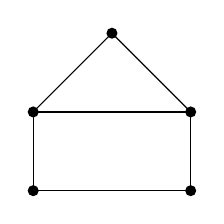
\begin{tikzpicture}
    % define variables.
    \def\a{(1,2)}
    \def\b{(0,1)}
    \def\c{(2,1)}
    \def\d{(0,0)}
    \def\e{(2,0)}
    % draw the vertices
    \fill \a circle (2pt);
    \fill \b circle (2pt);
    \fill \c circle (2pt);
    \fill \d circle (2pt);
    \fill \e circle (2pt);
    % draw the edges
    \draw \a -- \b;
    \draw \b -- \c;
    \draw \c -- \a;
    \draw \b -- \d;
    \draw \c -- \e;
    \draw \d -- \e;
\end{tikzpicture}}


\def\petersen{
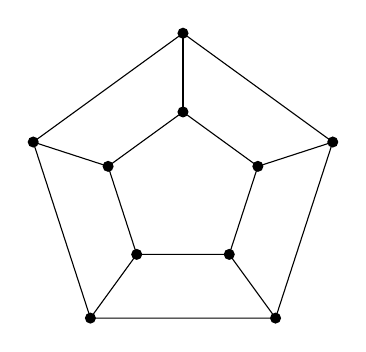
\begin{tikzpicture}
    \draw (18:2cm) -- (90:2cm) -- (162:2cm) -- (234:2cm) -- (306:2cm) -- cycle;
    \draw (18:1cm) -- (90:1cm) -- (162:1cm) -- (234:1cm) -- (306:1cm) -- cycle;
    \foreach \x in {18,90,162,234,306}{
        \draw (\x:1cm) -- (\x:2cm);
        \fill (\x:1cm) circle (2pt);
        \fill (\x:2cm) circle (2pt);
    }
\end{tikzpicture}
}

\def\kfive{
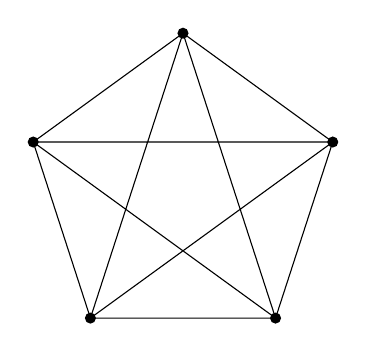
\begin{tikzpicture}
    \draw (18:2cm) -- (90:2cm) -- (162:2cm) -- (234:2cm) -- (306:2cm) -- cycle;
    \draw (18:2cm) -- (162:2cm) -- (306:2cm) -- (90:2cm) -- (234:2cm) -- cycle;
    \foreach \x in {18,90,162,234,306}{
        \fill (\x:2cm) circle (2pt);
    }
\end{tikzpicture}
}

\def\kthreetwo{
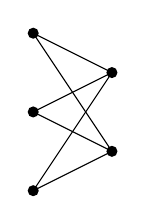
\begin{tikzpicture}
    % define variables.
    \def\a{(1,0.5)}
    \def\b{(1,1.5)}
    \def\c{(0,0)}
    \def\d{(0,1)}
    \def\e{(0,2)}
    % draw the vertices
    \fill \a circle (2pt);
    \fill \b circle (2pt);
    \fill \c circle (2pt);
    \fill \d circle (2pt);
    \fill \e circle (2pt);
    % draw the edges
    \draw \a -- \c;
    \draw \a -- \d;
    \draw \a -- \e;
    \draw \b -- \c;
    \draw \b -- \d;
    \draw \b -- \e;
\end{tikzpicture}}

\begin{enumerate}

  \item
given an empty heap perform the following operations.\\
Give the state of the heap (draw the tree) at each step.\\
push 1 \\
push 5 \\
push 3 \\
push 4 \\
push 2 \\
pop \\
pop \\
pop \\
pop \\
pop \\
$\ $\\
What order do the nodes come out in?\\
If I were to do this with $n$ elements, what's the total running time?\\

\newpage

\item

  \begin{enumerate}[itemsep=4em]
    \item Give an algorithm to find the sum of all of the elements in a linked list.
    \item Give an algorithm to count the number of nodes in a binary tree.
    \item Give an algorithm to find the smallest number in a linked list.
    \item Give an algorithm to find the smallest number in a binary tree.
  \end{enumerate}

\newpage

\item

Use structural induction to prove that:
\begin{enumerate}
  \item for linked lists: $count(a + b) = count(a) + count(b)$

  \item for trees: $height(mirror(t)) = height(t)$
\end{enumerate}

%%%%%%%%%%%%%
  \newpage %%%%%%%%%%%%%%%%%%%%%%%%%%%%%%%%%%%%%%%%%%%%%%%%%%%%%%%%%%%%%%%%%%%%
%%%%%%%%%%%%%

\item

Given a graph $G$, we can define a relation $\rightsquigarrow$ where
$u \rightsquigarrow v$ if there's a path from $u$ to $v$ in $G$.\\
Show that $\rightsquigarrow$ is an equivalence relation.

%%%%%%%%%%%%%
  \newpage %%%%%%%%%%%%%%%%%%%%%%%%%%%%%%%%%%%%%%%%%%%%%%%%%%%%%%%%%%%%%%%%%%%%
%%%%%%%%%%%%%

\item

Give An adjacency list, adjacency matrix, and edge list for the following graphs.

\begin{enumerate}[itemsep=6em]
  \item $\ $\\ \house

  \item $\ $\\ \petersen

%%%%%%%%%%%%%
  \newpage %%%%%%%%%%%%%%%%%%%%%%%%%%%%%%%%%%%%%%%%%%%%%%%%%%%%%%%%%%%%%%%%%%%%
%%%%%%%%%%%%%

  \item $\ $\\ \kfive

  \item $\ $\\ \kthreetwo

\end{enumerate}

\end{enumerate}


\end{document}
